%===================================================================================
\chapter{General Use Linear Solver Components in SUNDIALS}\label{s:gen_linsolv}
%===================================================================================

In this chapter, we describe linear solver code components that are included in
{\sundials}, but which are of potential use as generic packages in themselves,
either in conjunction with the use of {\sundials} or separately.

These generic modules in {\sundials} are organized in
three families, the {\em dls} family, which includes direct
linear solvers appropriate for sequential computations; the {\em sls}
family, which includes sparse matrix solvers; and the {\em spils}
family, which includes scaled preconditioned iterative (Krylov) linear solvers.
The solvers in each family share common data structures and functions.

The {\em dls} family contains the following two generic linear solvers:
\begin{itemize}
\item The {\dense} package, a linear solver for dense matrices either specified 
  through a matrix type (defined below) or as simple arrays.
\item The {\band} package, a linear solver for banded matrices either specified 
  through a matrix type (defined below) or as simple arrays.
\end{itemize}
Note that this family also includes the Blas/Lapack linear solvers (dense and band) 
available to the {\sundials} solvers, but these are not discussed here.

The {\em sls} family contains a sparse matrix package and interfaces between
it and two sparse direct solver packages:
\begin{itemize}
\item The {\klu} package, a linear solver for compressed-sparse-column
  matrices, \cite{KLU_site,DaPa:10}.
\item The {\superlumt} package, a threaded linear solver for
  compressed-sparse-column matrices, \cite{SuperLUMT_site,Li:05,DGL:99}.
\end{itemize}

The {\em spils} family contains the following generic linear solvers:
\begin{itemize}
\item The {\spgmr} package, a solver for the scaled preconditioned GMRES method.
\item The {\spfgmr} package, a solver for the scaled preconditioned Flexible GMRES method.
\item The {\spbcg} package, a solver for the scaled preconditioned Bi-CGStab method.
\item The {\sptfqmr} package, a solver for the scaled preconditioned TFQMR method.
\end{itemize}

For reasons related to installation, the names of the files involved
in these packages begin with the prefix \id{sundials\_}.  But
despite this, each of the {\em dls} and {\em spils} solvers is in fact generic, 
in that it is usable completely independently of {\sundials}.

For the sake of space, the functions for the \id{dense} and \id{band} modules
that work with a matrix type, and the functions in the {\spgmr}, 
{\spfgmr}, {\spbcg}, and {\sptfqmr}
modules are only summarized briefly, since they are less likely to be of direct use
in connection with a {\sundials} solver.  However, the functions for dense matrices 
treated as simple arrays and sparse matrices are fully described,
because we expect that they will be 
useful in the implementation of preconditioners used with the combination of one of
the {\sundials} solvers and one of the {\em spils} linear solvers.


% ====================================================================================
\section{The DLS modules: DENSE and BAND}\label{s:dls}
% ====================================================================================

\index{generic linear solvers!DENSE@{\dense}}
\index{generic linear solvers!BAND@{\band}}
The files comprising the {\dense} generic linear solver, and their locations
in the {\sundials} {\em srcdir}, are as follows:
\begin{itemize}
\item header files (located in {\em srcdir}\id{/include/sundials})\\
  \id{sundials\_direct.h}, \id{sundials\_dense.h}, \\
  \id{sundials\_types.h}, \id{sundials\_math.h},  \id{sundials\_config.h}
\item source files (located in {\em srcdir}\id{/src/sundials})\\
  \id{sundials\_direct.c}, \id{sundials\_dense.c}, \id{sundials\_math.c}
\end{itemize}
The files comprising the {\band} generic linear solver are as follows:
\begin{itemize}
\item header files (located in {\em srcdir}\id{/include/sundials})\\
  \id{sundials\_direct.h}, \id{sundials\_band.h}, \\
  \id{sundials\_types.h}, \id{sundials\_math.h},  \id{sundials\_config.h}
\item source files (located in {\em srcdir}\id{/src/sundials})\\
  \id{sundials\_direct.c}, \id{sundials\_band.c}, \id{sundials\_math.c}
\end{itemize}
%%
Only two of the preprocessing directives in the header file \id{sundials\_config.h} 
are relevant to the {\dense} and {\band} packages by themselves.
\begin{itemize}
\item (required) definition of the precision of the {\sundials} type \id{realtype}. 
  One of the following lines must be present:\\
  \id{\#define SUNDIALS\_DOUBLE\_PRECISION 1}\\
  \id{\#define SUNDIALS\_SINGLE\_PRECISION 1}\\
  \id{\#define SUNDIALS\_EXTENDED\_PRECISION 1}
\item (optional) use of generic math functions:
  \id{\#define SUNDIALS\_USE\_GENERIC\_MATH 1}
\end{itemize}
The \id{sundials\_types.h} header file defines the {\sundials} \id{realtype} and
\id{booleantype} types and the macro \id{RCONST}, while the \id{sundials\_math.h}
header file is needed for the macros \id{SUNMIN} and \id{SUNMAX}, and the
function \id{SUNRabs}.

The files listed above for either module can be extracted  from the {\sundials} 
{\em srcdir} and compiled by themselves into a separate library or into a larger user code.

% ------------------------------------------------------------------------------
\subsection{Type DlsMat}
% ------------------------------------------------------------------------------
%%
\index{DENSE@{\dense} generic linear solver!type \id{DlsMat}|(}
\index{BAND@{\band} generic linear solver!type \id{DlsMat}|(}
The type \ID{DlsMat}, defined in \id{sundials\_direct.h} is a pointer to a 
structure defining a generic matrix, and is used with all linear solvers in 
the {\em dls} family:
\begin{verbatim}
typedef struct _DlsMat {
  int type;
  long int M;
  long int N;
  long int ldim;
  long int mu;
  long int ml;
  long int s_mu;
  realtype *data;
  long int ldata;
  realtype **cols;
} *DlsMat;
\end{verbatim}
%%
For the {\dense} module, the relevant fields of this structure are as follows.
Note that a dense matrix of type \id{DlsMat} need not be square.
\begin{description}
  \item[type]  - \id{SUNDIALS\_DENSE} (=1)
  \item[M]  - number of rows
  \item[N]  - number of columns
  \item[ldim]  - leading dimension (\id{ldim} $\ge$ \id{M})
  \item[data]  - pointer to a contiguous block of \id{realtype} variables
  \item[ldata] - length of the data array ($=$ \id{ldim}$\cdot$\id{N}).
    The (\id{i},\id{j})-th element of a dense matrix \id{A} of type \id{DlsMat}
    (with $0 \le$ \id{i} $<$ \id{M} and $ 0 \le$ \id{j} $<$ \id{N}) 
    is given by the expression \id{(A->data)[0][j*M+i]}
  \item[cols]  - array of pointers. \id{cols[j]} points to the first element 
    of the j-th column of the matrix in the array data.
    The (\id{i},\id{j})-th element of a dense matrix \id{A} of type \id{DlsMat}
    (with $0 \le$ \id{i} $<$ \id{M} and $ 0 \le$ \id{j} $<$ \id{N}) 
    is given by the expression \id{(A->cols)[j][i]} 
\end{description}
%%
For the {\band} module, the relevant fields of this structure are as follows
(see Figure \ref{f:bandmat} for a diagram of the underlying data representation
in a banded matrix of type \id{DlsMat}). Note that only square band matrices are 
allowed.
\begin{description}
  \item[type]  - \id{SUNDIALS\_BAND} (=2)
  \item[M]  - number of rows
  \item[N]  - number of columns (\id{N} = \id{M})
  \item[mu]    - upper half-bandwidth, $0 \le$ \id{mu} $<$ min(\id{M},\id{N})
  \item[ml]    - lower half-bandwidth, $0 \le$ \id{ml} $<$ min(\id{M},\id{N})
  \item[s\_mu]  - storage upper bandwidth, \id{mu} $\le$ \id{s\_mu} $<$ \id{N}.
    The LU decomposition routine writes the LU factors into the storage 
    for A. The upper triangular factor U, however, may have 
    an upper bandwidth as big as min(\id{N}-1,\id{mu}+\id{ml}) because of 
    partial pivoting. The \id{s\_mu} field holds the upper half-bandwidth allocated for A.
  \item[ldim]  - leading dimension (\id{ldim} $\ge$ \id{s\_mu})
  \item[data]  - pointer to a contiguous block of \id{realtype} variables.
    The elements of a banded matrix of type \id{DlsMat} are      
    stored columnwise (i.e. columns are stored one on top  
    of the other in memory). Only elements within the      
    specified half-bandwidths are stored.     
    \id{data} is a pointer to \id{ldata} contiguous locations   
    which hold the elements within the band of A.  
  \item[ldata] - length of the data array ($=$ \id{ldim}$\cdot$(\id{s\_mu}+\id{ml}+1)
  \item[cols]  - array of pointers. \id{cols[j]} is a pointer to the uppermost element 
    within the band  in the j-th column. This pointer may be treated as   
    an array indexed from \id{s\_mu}$-$\id{mu} (to access the uppermost element within the 
    band in the j-th column) to \id{s\_mu}$+$\id{ml} (to access the lowest element     
    within the band in the j-th column). Indices from $0$ to \id{s\_mu}$-$\id{mu}$-1$ give 
    access to extra storage elements required by the LU decomposition function.
    Finally, \id{cols[j][i-j+s\_mu]} is the $(i,j)$-th element, $j-$\id{mu} $\le i \le j+$\id{ml}. 
\end{description}
%%
%%
\begin{figure}
\centerline{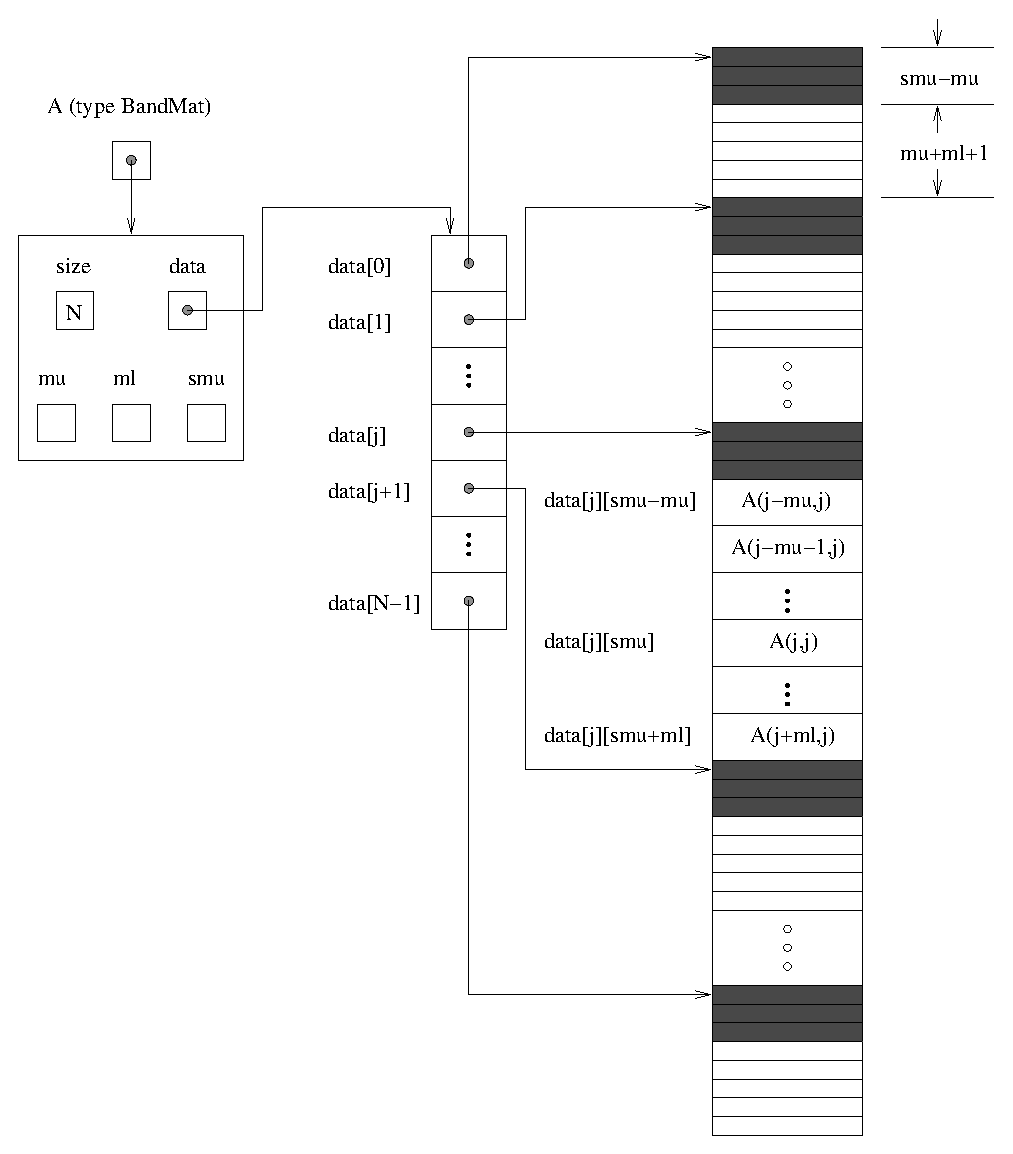
\includegraphics[width=4.5 in]{bandmat}}
\caption[Diagram of the storage for a banded matrix of type \id{DlsMat}]
  {Diagram of the storage for a banded matrix of type \id{DlsMat}. Here \id{A} is an
  $N \times N$ band matrix of type \id{DlsMat} with upper and lower half-bandwidths \id{mu}
  and \id{ml}, respectively. The rows and columns of \id{A} are numbered from $0$ to $N-1$
  and the ($i,j$)-th element of \id{A} is denoted \id{A(i,j)}. The greyed out areas of
  the underlying component storage are used by the \id{BandGBTRF} and
  \id{BandGBTRS} routines.}\label{f:bandmat}
\end{figure}
%%
%%

% ------------------------------------------------------------------------------
\subsection{Accessor macros for the DLS modules}
% ------------------------------------------------------------------------------

The macros below allow a user to efficiently access individual matrix           
elements without writing out explicit data structure           
references and without knowing too much about the underlying   
element storage. The only storage assumption needed is that    
elements are stored columnwise and that a pointer to the \id{j}-th 
column of elements can be obtained via the \id{DENSE\_COL} or \id{BAND\_COL} macros.    
Users should use these macros whenever possible.               
\index{BAND@{\band} generic linear solver!type \id{DlsMat}|)}
\index{DENSE@{\dense} generic linear solver!type \id{DlsMat}|)}

\index{DENSE@{\dense} generic linear solver!macros|(}
The following two macros are defined by the {\dense} module to provide
access to data in the \id{DlsMat} type:
\begin{itemize}
\item \ID{DENSE\_ELEM}
  \par Usage : \id{DENSE\_ELEM(A,i,j) = a\_ij;} or
  \id{a\_ij = DENSE\_ELEM(A,i,j);}
  \par \id{DENSE\_ELEM} references the (\id{i},\id{j})-th element of the $M \times N$
  \id{DlsMat} \id{A}, $0 \le$ \id{i} $< M$, $0 \le$ \id{j} $< N$.
  
\item \ID{DENSE\_COL}
  \par Usage : \id{col\_j = DENSE\_COL(A,j);}
  \par \id{DENSE\_COL} references the \id{j}-th column of the $M \times N$
  \id{DlsMat} \id{A}, $0 \le$ \id{j} $< N$. The type of the expression          
  \id{DENSE\_COL(A,j)} is \id{realtype *} . After the assignment in the usage    
  above, \id{col\_j} may be treated as an array indexed from $0$ to $M-1$. 
  The (\id{i}, \id{j})-th element of \id{A} is referenced by \id{col\_j[i]}.  
\end{itemize}
\index{DENSE@{\dense} generic linear solver!macros|)}

\index{BAND@{\band} generic linear solver!macros|(}
The following three macros are defined by the {\band} module to provide
access to data in the \id{DlsMat} type:
\begin{itemize}
\item \ID{BAND\_ELEM}
  \par Usage : \id{BAND\_ELEM(A,i,j) = a\_ij;} or \id{a\_ij = BAND\_ELEM(A,i,j);}
  \par \id{BAND\_ELEM} references the (\id{i},\id{j})-th element of the
  $N \times N$ band matrix \id{A}, where $0 \le$ \id{i}, \id{j} $\le N-1$.
  The location (\id{i},\id{j}) should further satisfy 
  \id{j}$-$\id{(A->mu)} $\le$ \id{i} $\le$ \id{j}$+$\id{(A->ml)}.
\item \ID{BAND\_COL}
  \par Usage : \id{col\_j = BAND\_COL(A,j);}
  \par \id{BAND\_COL} references the diagonal element of the \id{j}-th
  column of the $N \times N$ band matrix \id{A}, $0 \le$ \id{j} $\le N-1$.
  The type of the expression \id{BAND\_COL(A,j)} is \id{realtype *}. 
  The pointer returned by the call \id{BAND\_COL(A,j)} can be treated as 
  an array which is indexed from $-$\id{(A->mu)} to \id{(A->ml)}.
\item \ID{BAND\_COL\_ELEM}
  \par Usage : \id{BAND\_COL\_ELEM(col\_j,i,j) = a\_ij;} or
  \id{a\_ij = BAND\_COL\_ELEM(col\_j,i,j);}
  \par This macro references the (\id{i},\id{j})-th entry of the band matrix \id{A}
  when used in conjunction with \id{BAND\_COL} to reference the \id{j}-th column through
  \id{col\_j}. The index (\id{i},\id{j}) should satisfy 
  \id{j}$-$\id{(A->mu)} $\le$ \id{i} $\le$ \id{j}$+$\id{(A->ml)}.
\end{itemize}
\index{BAND@{\band} generic linear solver!macros|)}



% ------------------------------------------------------------------------------
\subsection{Functions in the DENSE module}\label{ss:dense}
% ------------------------------------------------------------------------------

The {\dense} module defines two sets of functions with corresponding names.
The first set contains functions (with names starting with a capital letter)
that act on dense matrices of type \id{DlsMat}.  The second set contains functions
(with names starting with a lower case letter) that act on matrices represented 
as simple arrays.

\index{DENSE@{\dense} generic linear solver!functions!large matrix|(}
The following functions for \id{DlsMat} dense matrices are available
in the {\dense} package.  For full details, see the header files
\id{sundials\_direct.h} and \id{sundials\_dense.h}.
\begin{itemize}
\item \id{NewDenseMat}: allocation of a \id{DlsMat} dense matrix;
\item \id{DestroyMat}: free memory for a \id{DlsMat} matrix;
\item \id{PrintMat}: print a \id{DlsMat} matrix to standard output.
\item \id{NewLintArray}: allocation of an array of \id{long int} integers for use
  as pivots with \id{DenseGETRF} and \id{DenseGETRS};
\item \id{NewIntArray}: allocation of an array of \id{int} integers for use
  as pivots with the Lapack dense solvers;
\item \id{NewRealArray}: allocation of an array of \id{realtype} for use
  as right-hand side with \id{DenseGETRS};
\item \id{DestroyArray}: free memory for an array;
\item \id{SetToZero}: load a matrix with zeros;
\item \id{AddIdentity}: increment a square matrix by the identity matrix;
\item \id{DenseCopy}: copy one matrix to another;
\item \id{DenseScale}: scale a matrix by a scalar;
\item \id{DenseGETRF}: LU factorization with partial pivoting;
\item \id{DenseGETRS}: solution of $Ax = b$ using LU factorization (for square matrices $A$);
\item \id{DensePOTRF}: Cholesky factorization of a real symmetric positive matrix;
\item \id{DensePOTRS}: solution of $Ax = b$ using the Cholesky factorization of $A$;
\item \id{DenseGEQRF}: QR factorization of an $m \times n$ matrix, with $m \ge n$;
\item \id{DenseORMQR}: compute the product $w = Qv$, with $Q$ calculated using \id{DenseGEQRF};
\item \id{DenseMatvec}: compute the product $y = Ax$, for an $M$ by $N$ matrix $A$;
\end{itemize}
\index{DENSE@{\dense} generic linear solver!functions!large matrix|)}

\index{DENSE@{\dense} generic linear solver!functions!small matrix|(}
The following functions for small dense matrices are available in the
{\dense} package:
%
\begin{itemize}

\item \ID{newDenseMat}
  \par \id{newDenseMat(m,n)} allocates storage for an \id{m} by \id{n}
  dense matrix. It returns a pointer to the newly allocated storage if            
  successful. If the memory request cannot be satisfied, then    
  \id{newDenseMat} returns \id{NULL}. The underlying type of the dense matrix 
  returned is \id{realtype**}. If we allocate a dense matrix \id{realtype** a} by 
  \id{a = newDenseMat(m,n)}, then \id{a[j][i]} references the (\id{i},\id{j})-th element   
  of the matrix \id{a}, $0 \le$ \id{i} $<$ \id{m}, $0 \le$ \id{j} $<n$, and \id{a[j]} 
  is a pointer to the first element in the \id{j}-th column of \id{a}. 
  The location \id{a[0]} contains a pointer to \id{m} $\times$ \id{n} contiguous 
  locations which contain the elements of \id{a}.

\item \ID{destroyMat}
  \par \id{destroyMat(a)} frees the dense matrix \id{a} allocated by \id{newDenseMat};

\item \ID{newLintArray}
  \par \id{newLintArray(n)} allocates an array of \id{n} integers, all \id{long int}.
  It returns a pointer to the first element in the array if successful. 
  It returns \id{NULL} if the memory request could not be satisfied.

\item \ID{newIntArray}
  \par \id{newIntArray(n)} allocates an array of \id{n} integers, all \id{int}.
  It returns a pointer to the first element in the array if successful. 
  It returns \id{NULL} if the memory request could not be satisfied.

\item \ID{newRealArray}
  \par \id{newRealArray(n)} allocates an array of \id{n} \id{realtype} values. 
  It returns a pointer to the first element in the array if successful. 
  It returns \id{NULL} if the memory request could not be satisfied.

\item \ID{destroyArray}
  \par \id{destroyArray(p)} frees the array \id{p} allocated by \id{newLintArray},
  \id{newIntArray}, or \id{newRealArray};

\item \ID{denseCopy}
  \par \id{denseCopy(a,b,m,n)} copies the \id{m} by \id{n} dense matrix \id{a} into the
  \id{m} by \id{n} dense matrix \id{b};

\item \ID{denseScale}
  \par \id{denseScale(c,a,m,n)} scales every element in the \id{m} by \id{n} dense
  matrix \id{a} by the scalar \id{c};

\item \ID{denseAddIdentity}
  \par \id{denseAddIdentity(a,n)} increments the {\em square} \id{n} by \id{n} dense matrix 
  \id{a} by the identity matrix $I_n$;

\item \ID{denseGETRF}
  \par \id{denseGETRF(a,m,n,p)} factors the \id{m} by \id{n} dense matrix \id{a},
  using Gaussian elimination with row pivoting. 
  It overwrites the elements of \id{a} with its LU factors and keeps track of the
  pivot rows chosen in the pivot array \id{p}.

  A successful LU factorization leaves the matrix \id{a} and the      
  pivot array \id{p} with the following information:                  
  \begin{enumerate}
  \item 
    \id{p[k]} contains the row number of the pivot element chosen   
    at the beginning of elimination step \id{k}, 
    \id{k} $ = 0, 1, ..., $\id{n}$-1$.  

  \item 
    If the unique LU factorization of \id{a} is given by $Pa = LU$,   
    where $P$ is a permutation matrix, $L$ is an \id{m} by \id{n}
    lower trapezoidal matrix with all diagonal elements equal to $1$, 
    and $U$ is an \id{n} by \id{n} upper triangular matrix, 
    then the upper triangular part of \id{a} (including its diagonal) 
    contains $U$ and the strictly lower trapezoidal part of \id{a} 
    contains the multipliers, $I-L$. 
    If \id{a} is square, $L$ is a unit lower triangular matrix.
                      
    \id{denseGETRF} returns 0 if successful. Otherwise it encountered a zero  
    diagonal element during the factorization, indicating that the matrix \id{a}
    does not have full column rank.
    In this case it returns the column index (numbered from one) at which it       
    encountered the zero.
    \end{enumerate}

\item \ID{denseGETRS}
  \par \id{denseGETRS(a,n,p,b)} solves the \id{n} by \id{n} linear system $ax = b$. 
  It assumes that \id{a} (of size \id{n} $\times$ \id{n}) has been LU-factored 
  and the pivot array \id{p} has been set by a successful call to 
  \id{denseGETRF(a,n,n,p)}. The solution $x$ is written into the \id{b} array.

\item \ID{densePOTRF}
  \par \id{densePOTRF(a,m)} calculates the Cholesky decomposition of the \id{m} by \id{m}
  dense matrix \id{a}, assumed to be symmetric positive definite. Only the lower triangle
  of \id{a} is accessed and overwritten with the Cholesky factor.

\item \ID{densePOTRS}
  \par \id{densePOTRS(a,m,b)} solves the \id{m} by \id{m} linear system $ax = b$.
  It assumes that the Cholesky factorization of \id{a} has been calculated in the
  lower triangular part of \id{a} by a successful call to \id{densePOTRF(a,m)}.

\item \ID{denseGEQRF}
  \par \id{denseGEQRF(a,m,n,beta,wrk)} calculates the QR decomposition of the \id{m} by \id{n}
  matrix \id{a} (\id{m} $\ge$ \id{n}) using Householder reflections. On exit, the elements
  on and above the diagonal of \id{a} contain the \id{n} by \id{n} upper triangular matrix \id{R};
  the elements below the diagonal, with the array \id{beta}, represent the orthogonal matrix \id{Q}
  as a product of elementary reflectors. The real array \id{wrk}, of length \id{m}, must be provided
  as temporary workspace.

\item \ID{denseORMQR}
  \par \id{denseORMQR(a,m,n,beta,v,w,wrk)} calculates the product $w = Qv$ for a given vector
  \id{v} of length \id{n}, where the orthogonal matrix $Q$ is encoded in the \id{m} by \id{n}
  matrix \id{a} and the vector \id{beta} of length \id{n}, after a successful call to
  \id{denseGEQRF(a,m,n,beta,wrk)}. The real array \id{wrk}, of length \id{m}, must be provided
  as temporary workspace.

\item \ID{denseMatvec}
  \par \id{denseMatvec(a,x,y,m,n)} calculates the product $y = ax$ for a given vector
  \id{x} of length \id{n}, and \id{m} by \id{n} matrix \id{a}.

\end{itemize}
\index{DENSE@{\dense} generic linear solver!functions!small matrix|)}


% ------------------------------------------------------------------------------
\subsection{Functions in the BAND module}\label{ss:band}
% ------------------------------------------------------------------------------

The {\band} module defines two sets of functions with corresponding names.
The first set contains functions (with names starting with a capital letter)
that act on band matrices of type \id{DlsMat}.  The second set contains functions
(with names starting with a lower case letter) that act on matrices represented 
as simple arrays.

\index{BAND@{\band} generic linear solver!functions|(}
The following functions for \id{DlsMat} banded matrices are available
in the {\band} package.  For full details, see the header files
\id{sundials\_direct.h} and \id{sundials\_band.h}.
\begin{itemize}
\item \id{NewBandMat}: allocation of a \id{DlsMat} band matrix;
\item \id{DestroyMat}: free memory for a \id{DlsMat} matrix;
\item \id{PrintMat}: print a \id{DlsMat} matrix to standard output.
\item \id{NewLintArray}: allocation of an array of \id{int} integers for use
  as pivots with \id{BandGBRF} and \id{BandGBRS};
\item \id{NewIntArray}: allocation of an array of \id{int} integers for use
  as pivots with the Lapack band solvers;
\item \id{NewRealArray}: allocation of an array of \id{realtype} for use
  as right-hand side with \id{BandGBRS};
\item \id{DestroyArray}: free memory for an array;
\item \id{SetToZero}: load a matrix with zeros;
\item \id{AddIdentity}: increment a square matrix by the identity matrix;
\item \id{BandCopy}: copy one matrix to another;
\item \id{BandScale}: scale a matrix by a scalar;
\item \id{BandGBTRF}: LU factorization with partial pivoting;
\item \id{BandGBTRS}: solution of $Ax = b$ using LU factorization;
\item \id{BandMatvec}: compute the product $y = Ax$, for a square band matrix $A$;
\end{itemize}
\index{BAND@{\band} generic linear solver!functions|)}

\index{BAND@{\band} generic linear solver!functions!small matrix|(}
The following functions for small band matrices are available in the
{\band} package:
\begin{itemize}

\item \ID{newBandMat}
  \par \id{newBandMat(n, smu, ml)} allocates storage for an \id{n} by \id{n}
  band matrix with lower half-bandwidth \id{ml}.

\item \ID{destroyMat}
  \par \id{destroyMat(a)} frees the band matrix \id{a} allocated by \id{newBandMat};

\item \ID{newLintArray}
  \par \id{newLintArray(n)} allocates an array of \id{n} integers, all \id{long int}. 
  It returns a pointer to the first element in the array if successful. 
  It returns \id{NULL} if the memory request could not be satisfied.

\item \ID{newIntArray}
  \par \id{newIntArray(n)} allocates an array of \id{n} integers, all \id{int}.
  It returns a pointer to the first element in the array if successful. 
  It returns \id{NULL} if the memory request could not be satisfied.

\item \ID{newRealArray}
  \par \id{newRealArray(n)} allocates an array of \id{n} \id{realtype} values. 
  It returns a pointer to the first element in the array if successful. 
  It returns \id{NULL} if the memory request could not be satisfied.

\item \ID{destroyArray}
  \par \id{destroyArray(p)} frees the array \id{p} allocated by \id{newLintArray},
  \id{newIntArray}, or \id{newRealArray};

\item \ID{bandCopy}
  \par \id{bandCopy(a,b,n,a\_smu, b\_smu,copymu, copyml)} copies the \id{n} by \id{n} band 
  matrix \id{a} into the \id{n} by \id{n} band matrix \id{b};

\item \ID{bandScale}
  \par \id{bandScale(c,a,n,mu,ml,smu)} scales every element in the \id{n} by \id{n} band
  matrix \id{a} by \id{c};

\item \ID{bandAddIdentity}
  \par \id{bandAddIdentity(a,n,smu)} increments the \id{n} by \id{n} band matrix \id{a} by the
  identity matrix;

\item \ID{bandGETRF}
  \par \id{bandGETRF(a,n,mu,ml,smu,p)} factors the \id{n} by \id{n} band matrix \id{a},
  using Gaussian elimination with row pivoting. 
  It overwrites the elements of \id{a} with its LU factors and keeps track of the
  pivot rows chosen in the pivot array \id{p}.

\item \ID{bandGETRS}
  \par \id{bandGETRS(a,n,smu,ml,p,b)} solves the \id{n} by \id{n} linear system $ax = b$. 
  It assumes that \id{a} (of size \id{n} $\times$ \id{n}) has been LU-factored 
  and the pivot array \id{p} has been set by a successful call to 
  \id{bandGETRF(a,n,mu,ml,smu,p)}. The solution $x$ is written into the \id{b} array.

\item \ID{bandMatvec}
  \par \id{bandMatvec(a,x,y,n,mu,ml,smu)} calculates the product $y = ax$ for a given vector
  \id{x} of length \id{n}, and \id{n} by \id{n} band matrix \id{a}.

\end{itemize}
\index{BAND@{\band} generic linear solver!functions!small matrix|)}


% ====================================================================================
\section{The SLS module}\label{s:sls}
% ====================================================================================

\index{generic linear solvers!SLS@{\sls}}
\index{generic linear solvers!KLU@{\klu}}
\index{generic linear solvers!SUPERLUMT@{\superlumt}}
{\sundials} provides a compressed-sparse-column matrix type and sparse
matrix support functions.  In addition, {\sundials} provides interfaces
to the publically available KLU and SuperLU\_MT sparse direct solver packages.
The files comprising the {\sls} matrix module, used in the {\klu} and
{\superlumt} linear solver packages, and their locations
in the {\sundials} {\em srcdir}, are as follows:
\begin{itemize}
\item header files (located in {\em srcdir}\id{/include/sundials})\\
  \id{sundials\_sparse.h}, \id{sundials\_klu\_impl.h}, \\
  \id{sundials\_superlumt\_impl.h}, \id{sundials\_types.h}, \\
  \id{sundials\_math.h},  \id{sundials\_config.h}
\item source files (located in {\em srcdir}\id{/src/sundials})\\
  \id{sundials\_sparse.c}, \id{sundials\_math.c}
\end{itemize}
%%
Only two of the preprocessing directives in the header file \id{sundials\_config.h} 
are relevant to the {\sls} package by itself:
\begin{itemize}
\item (required) definition of the precision of the {\sundials} type \id{realtype}. 
  One of the following lines must be present:\\
  \id{\#define SUNDIALS\_DOUBLE\_PRECISION 1}\\
  \id{\#define SUNDIALS\_SINGLE\_PRECISION 1}\\
  \id{\#define SUNDIALS\_EXTENDED\_PRECISION 1}
\item (optional) use of generic math functions:
  \id{\#define SUNDIALS\_USE\_GENERIC\_MATH 1}
\end{itemize}
The \id{sundials\_types.h} header file defines the {\sundials} \id{realtype} and
\id{booleantype} types and the macro \id{RCONST}, while the \id{sundials\_math.h}
header file is needed for the macros \id{SUNMIN} and \id{SUNMAX}, and the
function \id{SUNRabs}.

% ------------------------------------------------------------------------------
\subsection{Type SlsMat}
% ------------------------------------------------------------------------------
%%
\index{KLU@{\klu} sparse linear solver!type \id{SlsMat}|(}
\index{SUPERLUMT@{\superlumt} sparse linear solver!type \id{SlsMat}|(}
{\sundials} supports operations with matrices in compressed-sparse-column (CSC)
format and in compressed-sparse-row (CSR) format. For convenience, integer sparse 
matrix identifiers are defined as:\\
  \indent \id{\#define CSC\_MAT 0}\\
  \indent \id{\#define CSR\_MAT 1}\\
The type \ID{SlsMat}, defined in \id{sundials\_sparse.h} is a pointer to a 
structure defining generic CSC and CSR matrix formats, and is
used with all linear solvers in the {\em sls} family:
\begin{verbatim}
typedef struct _SlsMat {
  int M;
  int N;
  int NNZ;
  int NP;
  realtype *data;
  int sparsetype;
  int *indexvals;
  int *indexptrs;
  int **rowvals;
  int **colptrs;
  int **colvals;
  int **rowptrs;
} *SlsMat;
\end{verbatim}
%%
The fields of this structure are as follows (see Figure \ref{f:cscmat}
for a diagram of the underlying compressed-sparse-column
representation in a sparse matrix of type \id{SlsMat}).  Note that a
sparse matrix of type \id{SlsMat} need not be square.
\begin{description}
  \item[M]  - number of rows
  \item[N]  - number of columns
  \item[NNZ]  - maximum number of nonzero entries in the matrix
    (allocated length of \id{data} and \id{rowvals} arrays)
  \item[NP]  - number of index pointers (e.g. number of column pointers for 
    CSC matrix). For CSC matrices $NP=N$, and for CSR matrices $NP=M$. This 
    value is set automatically based the input for \verb|sparsetype|. 
  \item[data]  - pointer to a contiguous block of \id{realtype}
    variables (of length \id{NNZ}), containing the values of the
    nonzero entries in the matrix
  \item[sparsetype]  - type of the sparse matrix (\id{CSC\_MAT} or \id{CSR\_MAT})
  \item[indexvals] - pointer to a contiguous block of \id{int} variables
    (of length \id{NNZ}), containing the row indices (if CSC) or column
   indices (if CSR) of each nonzero matrix entry held in \id{data}
  \item[indexptrs]  - pointer to a contiguous block of \id{int}
    variables (of length \id{NP+1}). For CSC matrices each 
    entry provides the index of the first column entry into the 
    \id{data} and \id{indexvals} arrays, e.g. if \id{indexptr[3]=7}, then 
    the first nonzero entry in the fourth column of the matrix is 
    located in \id{data[7]}, and is located in row \id{indexvals[7]} of the 
    matrix.  The last entry contains the total number of nonzero values in 
    the matrix and hence points one past the end of the active data in the 
    \id{data} and \id{indexvals} arrays. For CSR matrices, each entry provides 
    the index of the first row entry into the \id{data} and \id{indexvals} 
    arrays.
\end{description}
\noindent The following pointers are added to the \id{SlsMat} type for user convenience, 
to provide a more intuitive interface to the CSC and CSR sparse matrix data structures. They are set 
automatically by the \id{SparseNewMat} function, based on the sparse matrix storage type. 
\begin{description}
  \item[rowvals] - pointer to \verb|indexvals| when \id{sparsetype} is \id{CSC\_MAT},
    otherwise set to \verb|NULL|.
  \item[colptrs] - pointer to \verb|indexptrs| when \id{sparsetype} is \id{CSC\_MAT},
    otherwise set to \verb|NULL|.
  \item[colvals] - pointer to \verb|indexvals| when \id{sparsetype} is \id{CSR\_MAT},
    otherwise set to \verb|NULL|.
  \item[rowptrs] - pointer to \verb|indexptrs| when \id{sparsetype} is \id{CSR\_MAT},
    otherwise set to \verb|NULL|.
\end{description}
For example, the $5\times 4$ CSC matrix
\[
  \left[\begin{array}{cccc} 
     0 & 3 & 1 & 0\\
     3 & 0 & 0 & 2\\
     0 & 7 & 0 & 0\\
     1 & 0 & 0 & 9\\
     0 & 0 & 0 & 5
  \end{array}\right]
\]
could be stored in a \id{SlsMat} structure as either
\begin{verbatim}
  M = 5;
  N = 4;
  NNZ = 8;
  NP = N;
  data = {3.0, 1.0, 3.0, 7.0, 1.0, 2.0, 9.0, 5.0};
  sparsetype = CSC_MAT;
  indexvals = {1, 3, 0, 2, 0, 1, 3, 4};
  indexptrs = {0, 2, 4, 5, 8};
  rowvals = &indexvals;
  colptrs = &indexptrs;
  colvals = NULL;
  rowptrs = NULL;
\end{verbatim}
or 
\begin{verbatim}
  M = 5;
  N = 4;
  NNZ = 10;
  NP = N;
  data = {3.0, 1.0, 3.0, 7.0, 1.0, 2.0, 9.0, 5.0, *, *};
  sparsetype = CSC_MAT;
  indexvals = {1, 3, 0, 2, 0, 1, 3, 4, *, *};
  indexptrs = {0, 2, 4, 5, 8};
  ...
\end{verbatim}
where the first has no unused space, and the second has additional
storage (the entries marked with \texttt{*} may contain any values).
Note in both cases that the final value in \id{indexptrs} is $8$.  The work 
associated with operations on the sparse matrix is proportional to this
value and so one should use the best understanding of the
number of nonzeroes here.
%%
%%
%%
\begin{figure}
\centerline{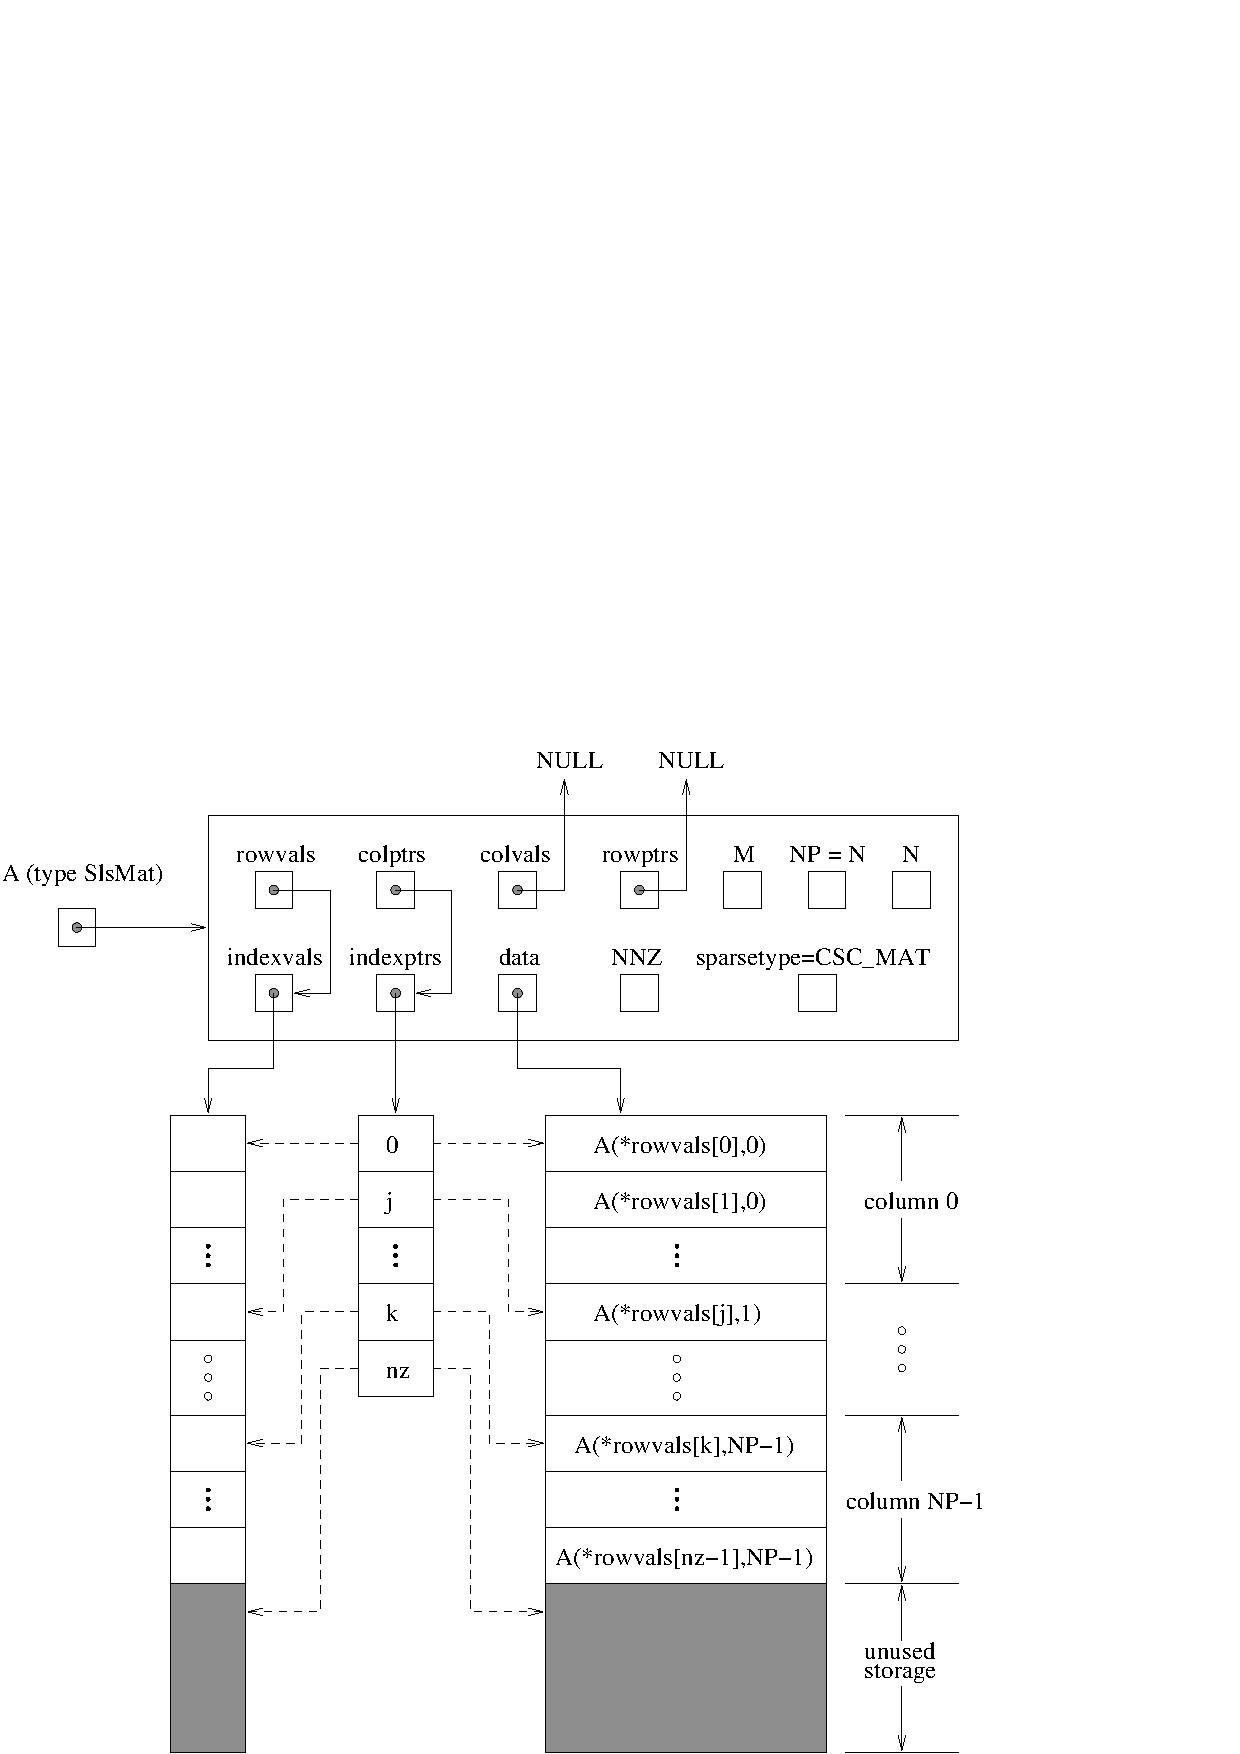
\includegraphics[width=4.5 in]{cscmat}}
\caption[Diagram of the storage for a compressed-sparse-column matrix
  of type \id{SlsMat}] 
  {Diagram of the storage for a compressed-sparse-column matrix of
  type \id{SlsMat}. Here \id{A} is an $M \times N$ sparse matrix of
  type \id{SlsMat} with storage for up to \id{NNZ} nonzero entries
  (the allocated length of both \id{data} and \id{indexvals}).  The
  entries in \id{indexvals} may assume values from $0$ to $M-1$,
  corresponding to the row index (zero-based) of each nonzero value.
  The entries in \id{data} contain the values of the nonzero entries,
  with the row $i$, column $j$ entry of \id{A} (again, zero-based)
  denoted as \id{A(i,j)}.  The \id{indexptrs} array contains $N+1$
  entries; the first $N$ denote the starting index of each column
  within the \id{indexvals} and \id{data} arrays, while the final entry
  points one past the final nonzero entry.  Here, although \id{NNZ}
  values are allocated, only \id{nz} are actually filled in; the
  greyed-out portions of \id{data} and \id{indexvals} indicate extra
  allocated space.}\label{f:cscmat}
\end{figure}
%%
%%

% ------------------------------------------------------------------------------
\subsection{Functions in the SLS module}\label{ss:sls_functions}
% ------------------------------------------------------------------------------

The {\sls} module defines functions that act on sparse matrices of
type \id{SlsMat}.  For full details, see the header file \id{sundials\_sparse.h}.
%
\index{SLS@{\sls} sparse linear solver!functions!small matrix|(}
\begin{itemize}

\item \ID{SparseNewMat}
  \par \id{SparseNewMat(M, N, NNZ, sparsetype)} allocates storage for an \id{M} by \id{N}
  sparse matrix, with storage for up to \id{NNZ} nonzero entries and \id{sparsetype} 
  storage type (\id{CSC\_MAT} or \id{CSR\_MAT}).

\item \ID{SparseFromDenseMat}
  \par \id{SparseFromDenseMat(A)} converts a dense or band matrix \id{A} of type
  \id{DlsMat} into a new CSC matrix of type \id{SlsMat} by retaining
  only the nonzero values of the matrix \id{A}.

\item \ID{SparseDestroyMat}
  \par \id{SparseDestroyMat(A)} frees the memory for a sparse matrix
  \id{A} allocated by either \id{SparseNewMat} or \id{SparseFromDenseMat}.

\item \ID{}
  \par \id{SparseSetMatToZero(A)} zeros out the \id{SlsMat} matrix \id{A}.
  The storage for \id{A} is left unchanged.

\item \ID{SparseCopyMat}
  \par \id{SparseCopyMat(A, B)} copies the \id{SlsMat} \id{A} into the
  \id{SlsMat} \id{B}.  It is assumed that the matrices have the same
  row/column dimensions and storage type.  If \id{B} has insufficient 
  storage to hold all the nonzero entries of \id{A}, the data and 
  index arrays in \id{B} are reallocated to match those in \id{A}.

\item \ID{SparseScaleMat}
  \par \id{SparseScaleMat(c, A)} scales every element in the
  \id{SlsMat} \id{A} by the \id{realtype} scalar \id{c}.

\item \ID{SparseAddIdentityMat}
  \par \id{SparseAddIdentityMat(A)} increments the \id{SlsMat} \id{A}
  by the identity matrix.  If \id{A} is not square, only the existing
  diagonal values are incremented.  Resizes the \id{data} and
  \id{rowvals} arrays of \id{A} to allow for new 
  nonzero entries on the diagonal.

\item \ID{SparseAddMat}
  \par \id{SparseAddMat(A, B)} adds two \id{SlsMat} matrices \id{A} and
  \id{B}, placing the result back in \id{A}.  Resizes the \id{data}
  and \id{rowvals} arrays of \id{A} upon completion to exactly match
  the nonzero storage for the result.  Upon successful completion, the
  return value is zero; otherwise -1 is returned. It is assumed that
  both matrices have the same size and storage type.

\item \ID{SparseReallocMat}
  \par \id{SparseReallocMat(A)} eliminates unused storage in the
  \id{SlsMat} \id{A} by resizing the internal \id{data} and
  \id{rowvals} arrays to contain exactly \id{colptrs[N]} values.

\item \ID{SparseMatvec}
  \par \id{SparseMatvec(A, x, y)} computes the sparse matrix-vector
  product, $y=Ax$.  If the \id{SlsMat} \id{A} 
  is a sparse matrix of dimension $M\times N$, then it is assumed
  that \id{x} is a \id{realtype} array of length $N$, and \id{y} is a
  \id{realtype} array of length $M$. Upon successful completion, the
  return value is zero; otherwise -1 is returned.

\item \ID{SparsePrintMat}
  \par \id{SparsePrintMat(A)} Prints the \id{SlsMat} matrix \id{A} to
  standard output.

\end{itemize}
\index{SLS@{\sls} sparse linear solver!functions!small matrix|)}



% ------------------------------------------------------------------------------
\subsection{The KLU solver}\label{ss:klu}
% ------------------------------------------------------------------------------

{\klu} is a sparse matrix factorization and solver library written by Tim
Davis \cite{KLU_site,DaPa:10}.  
{\klu} has a symbolic factorization routine that computes the permutation of 
the linear system matrix to block triangular form and the permutations that will 
pre-order the diagonal blocks (the only ones that need to be factored) to reduce 
fill-in (using AMD, COLAMD, CHOLAMD, natural, or an ordering given by the user).  
Note that SUNDIALS uses the COLAMD ordering by default with {\klu}.

{\klu} breaks the factorization into two separate parts.  The first is a symbolic
factorization and the second is a numeric 
factorization that returns the factored matrix along with final pivot information.  
{\klu} also has a refactor routine that can be called instead of the numeric 
factorization.  This routine will reuse the pivot information.  This routine 
also returns diagnostic information that a user can examine to determine if 
numerical stability is being lost and a full numerical factorization should 
be done instead of the refactor.  

The {\klu} interface in {\sundials} will perform the symbolic factorization once.
It then calls the numerical factorization once and will call the refactor routine
until estimates of the numerical conditioning suggest a new factorization 
should be completed.  The {\klu} interface also has a \id{ReInit} routine that 
can be used to force a full refactorization at the next solver setup call.

In order to use the {\sundials} interface to {\klu}, it is
assumed that {\klu} has been installed on the system prior to
installation of {\sundials}, and that {\sundials} has been configured
appropriately to link with {\klu} (see Appendix \ref{c:install} for details).

Designed for serial calculations only, {\klu} is supported for
calculations employing {\sundials}' serial or shared-memory parallel
{\nvector} modules (see Sections \ref{ss:nvec_ser}, \ref{ss:nvec_openmp}
and \ref{ss:nvec_pthreads} for details).

% ------------------------------------------------------------------------------
\subsection{The SUPERLUMT solver}\label{ss:superlumt}
% ------------------------------------------------------------------------------

{\superlumt} is a threaded sparse matrix factorization and solver
library written by X. Sherry Li \cite{SuperLUMT_site,Li:05,DGL:99}.  
The package performs matrix factorization using threads to enhance efficiency
in shared memory parallel environments.  It should be noted that threads are
only used in the factorization step.

In order to use 
the {\sundials} interface to {\superlumt}, it is assumed that {\superlumt}
has been installed on the system prior to installation of {\sundials}, and
that {\sundials} has been configured appropriately to link with
{\superlumt} (see Appendix \ref{c:install} for details).

Designed for serial and threaded calculations only, {\superlumt} is
supported for calculations employing {\sundials}' serial or shared-memory
parallel {\nvector} modules (see Sections \ref{ss:nvec_ser}, \ref{ss:nvec_openmp}
and \ref{ss:nvec_pthreads} for details).


% ====================================================================================
\section{The SPILS modules: SPGMR, SPFGMR, SPBCG, and SPTFQMR}\label{s:spils}
% ====================================================================================

The {\em spils} modules contain implementations of some of the most commonly
use scaled preconditioned Krylov solvers.
A linear solver module from the {\em spils} family can be used 
in conjunction with any {\nvector} implementation library.

% ------------------------------------------------------------------------------
\subsection{The SPGMR module}\label{ss:spgmr}
% ------------------------------------------------------------------------------

\index{generic linear solvers!SPGMR@{\spgmr}}
\index{SPGMR@{\spgmr} generic linear solver!description of|(}
The {\spgmr} package, in the files \id{sundials\_spgmr.h} and
\id{sundials\_spgmr.c}, includes an implementation of the scaled
preconditioned GMRES\index{GMRES method} method.  A separate code
module, implemented in \id{sundials\_iterative.(h,c)}, contains
auxiliary functions that support {\spgmr}, as well as the other Krylov
solvers in {\sundials} ({\spfgmr}, {\spbcg}, and {\sptfqmr}).
For full details, including usage instructions, see the header
files \id{sundials\_spgmr.h} and \id{sundials\_iterative.h}.
\index{SPGMR@{\spgmr} generic linear solver!description of|)}

The files comprising the {\spgmr} generic linear solver, and their locations
in the {\sundials} {\em srcdir}, are as follows:
\begin{itemize}
\item header files (located in {\em srcdir}\id{/include/sundials})\\
  \id{sundials\_spgmr.h}, \id{sundials\_iterative.h}, \id{sundials\_nvector.h}, \\
  \id{sundials\_types.h}, \id{sundials\_math.h},  \id{sundials\_config.h}
\item source files (located in {\em srcdir}\id{/src/sundials})\\
  \id{sundials\_spgmr.c}, \id{sundials\_iterative.c}, \id{sundials\_nvector.c}
\end{itemize}
Only two of the preprocessing directives in the header file \id{sundials\_config.h} 
are required to use the {\spgmr} package by itself:
\begin{itemize}
\item (required) definition of the precision of the {\sundials} type \id{realtype}. 
  One of the following lines must be present:\\
  \id{\#define SUNDIALS\_DOUBLE\_PRECISION 1}\\
  \id{\#define SUNDIALS\_SINGLE\_PRECISION 1}\\
  \id{\#define SUNDIALS\_EXTENDED\_PRECISION 1}
\item (optional) use of generic math functions:\\
  \id{\#define SUNDIALS\_USE\_GENERIC\_MATH 1}
\end{itemize}
The \id{sundials\_types.h} header file defines the {\sundials} \id{realtype} and
\id{booleantype} types and the macro \id{RCONST}, while the \id{sundials\_math.h}
header file is needed for the macros \id{SUNMIN}, \id{SUNMAX}, and \id{SUNSQR},
and the functions \id{SUNRabs} and \id{SUNRsqrt}.

The generic {\nvector} files, \id{sundials\_nvector.(h,c)} are needed for the
definition of the generic \id{N\_Vector} type and functions. 
The {\nvector} functions used by the {\spgmr} module are: 
\id{N\_VDotProd}, \id{N\_VLinearSum}, \id{N\_VScale}, \id{N\_VProd}, \id{N\_VDiv}, 
\id{N\_VConst}, \id{N\_VClone}, \id{N\_VCloneVectorArray}, \id{N\_VDestroy}, and
\id{N\_VDestroyVectorArray}.

The nine files listed above can be extracted from the {\sundials} {\em srcdir} and
compiled by themselves into an {\spgmr} library or into a larger user code.
 
\index{SPGMR@{\spgmr} generic linear solver!functions|(}
The following functions are available in the {\spgmr} package:  
\begin{itemize}
\item \id{SpgmrMalloc}: allocation of memory for \id{SpgmrSolve};
\item \id{SpgmrSolve}: solution of $Ax = b$ by the {\spgmr} method;
\item \id{SpgmrFree}: free memory allocated by \id{SpgmrMalloc}.
\end{itemize}
\index{SPGMR@{\spgmr} generic linear solver!functions|)}
%
\index{SPGMR@{\spgmr} generic linear solver!support functions|(}
The following functions are available in the support package 
\id{sundials\_iterative.(h,c)}:
\begin{itemize}
\item \id{ModifiedGS}: performs modified Gram-Schmidt procedure;
\item \id{ClassicalGS}: performs classical Gram-Schmidt procedure; 
\item \id{QRfact}: performs QR factorization of Hessenberg matrix;
\item \id{QRsol}: solves a least squares problem with a Hessenberg
       matrix factored by \id{QRfact}.
\end{itemize}
\index{SPGMR@{\spgmr} generic linear solver!support functions|)}


% ------------------------------------------------------------------------------
\subsection{The SPFGMR module}\label{ss:spfgmr}
% ------------------------------------------------------------------------------

\index{generic linear solvers!SPFGMR@{\spfgmr}}
\index{SPFGMR@{\spfgmr} generic linear solver!description of|(}
The {\spfgmr} package, in the files \id{sundials\_spfgmr.h} and
\id{sundials\_spfgmr.c}, includes an implementation of the scaled
preconditioned Flexible GMRES\index{FGMRES method} method.
For full details, including usage instructions, see the file \id{sundials\_spfgmr.h}.
\index{SPFGMR@{\spfgmr} generic linear solver!description of|)}

The files needed to use the {\spfgmr} module by itself are the same as for the
{\spgmr} module, but with \id{sundials\_spfgmr.(h,c)} in place of
\id{sundials\_spgmr.(h,c)}.

\index{SPFGMR@{\spfgmr} generic linear solver!functions|(}
The following functions are available in the {\spfgmr} package:  
\begin{itemize}
\item \id{SpfgmrMalloc}: allocation of memory for \id{SpfgmrSolve};
\item \id{SpfgmrSolve}: solution of $Ax = b$ by the {\spfgmr} method;
\item \id{SpfgmrFree}: free memory allocated by \id{SpfgmrMalloc}.
\end{itemize}
\index{SPFGMR@{\spfgmr} generic linear solver!functions|)}


% ------------------------------------------------------------------------------
\subsection{The SPBCG module}\label{ss:spbcg}
% ------------------------------------------------------------------------------

\index{generic linear solvers!SPBCG@{\spbcg}}
\index{SPBCG@{\spbcg} generic linear solver!description of|(}
The {\spbcg} package, in the files \id{sundials\_spbcgs.h} and
\id{sundials\_spbcgs.c}, includes an implementation of the scaled
preconditioned Bi-CGStab\index{Bi-CGStab method} method.
For full details, including usage instructions, see the file \id{sundials\_spbcgs.h}.
\index{SPBCG@{\spbcg} generic linear solver!description of|)}

The files needed to use the {\spbcg} module by itself are the same as for the
{\spgmr} module, but with \id{sundials\_spbcgs.(h,c)} in place of
\id{sundials\_spgmr.(h,c)}.

\index{SPBCG@{\spbcg} generic linear solver!functions|(}
The following functions are available in the {\spbcg} package:  
\begin{itemize}
\item \id{SpbcgMalloc}: allocation of memory for \id{SpbcgSolve};
\item \id{SpbcgSolve}: solution of $Ax = b$ by the {\spbcg} method;
\item \id{SpbcgFree}: free memory allocated by \id{SpbcgMalloc}.
\end{itemize}
\index{SPBCG@{\spbcg} generic linear solver!functions|)}



% ------------------------------------------------------------------------------
\subsection{The SPTFQMR module}\label{ss:sptfqmr}
% ------------------------------------------------------------------------------

\index{generic linear solvers!SPTFQMR@{\sptfqmr}}
\index{SPTFQMR@{\sptfqmr} generic linear solver!description of|(}
The {\sptfqmr} package, in the files \id{sundials\_sptfqmr.h} and
\id{sundials\_sptfqmr.c}, includes an implementation of the scaled
preconditioned TFQMR\index{TFQMR method} method.  For full details,
including usage instructions, see the file \id{sundials\_sptfqmr.h}.
\index{SPTFQMR@{\sptfqmr} generic linear solver!description of|)}

The files needed to use the {\sptfqmr} module by itself are the same as for the
{\spgmr} module, but with \id{sundials\_sptfqmr.(h,c)} in place of
\id{sundials\_spgmr.(h,c)}.

\index{SPTFQMR@{\sptfqmr} generic linear solver!functions|(}
The following functions are available in the {\sptfqmr} package:  
\begin{itemize}
\item \id{SptfqmrMalloc}: allocation of memory for \id{SptfqmrSolve};
\item \id{SptfqmrSolve}: solution of $Ax = b$ by the {\sptfqmr} method;
\item \id{SptfqmrFree}: free memory allocated by \id{SptfqmrMalloc}.
\end{itemize}
\index{SPTFQMR@{\sptfqmr} generic linear solver!functions|)}
